\documentclass{article}

% --- Packages ---
\usepackage[utf8]{inputenc} % Standard encoding
\usepackage{amsmath, amssymb, amsfonts} % Math symbols
\usepackage{graphicx} % For including figures
\usepackage{booktabs} % For professional-looking tables
\usepackage{hyperref} % For clickable links and cross-references
\usepackage[accepted]{../style/icml2025}


% --- Metadata ---
\title{Constructing An Environment Agnostic Tuberculosis Predictor From Ziehl-Neelsen Stained Sputum Smears Using A CNN}
\author{Nicholas Nolen}
\date{May 8, 2026}

\begin{document}

\maketitle

% --- Abstract ---
\begin{abstract}
% A brief overview of the paper.

Tuberculosis is one of the world's most infectious and deadly diseases. Tuberculosis affects about 25\%
of the world's population and is responsible for roughly 1.2 million deaths each year. In this work
I investigate using a CNN model to assist health officials in the diagnosis of Tuberculosis via likelihood classification of sputum
slides stained with the Ziehl-Neelsen staining technique. Through my methods I achieved a 0.9198
validation accuracy along with a 0.2097 binary cross-entropy validation loss and showed that the model I trained is likely
generalizable to other datasets and microscopy environments.
\end{abstract}

% --- Introduction ---
\section{Introduction}
% Describes the motivation of this work and outlines the rest of the paper.

According to the World Health Organization (WHO) approximately a quarter of the world's population is 
currently infected with Tuberculosis\cite{bai2024global}. In addition, the disease has been shown to be much more likely to 
have extreme adverse health impacts and be much harder to cure for those living in poverty. The best way to
prevent the spread of Tuberculosis in these places is being able to diagnose the disease early, however most diagnostic tools are very
expensive and the people living in these impoverished communities do not have access to them.

The current most widespread diagnostic tool for Tuberculosis in impoverished areas is manual Ziehl Neelsen stained sputum smear microscopy. The
Ziehl-Neelsen stain is used to detect Tuberculosis and other acid-fast bacteria which have a waxy lipid-rich outer layer
which causes them to be resistant to conventional staining techniques.
The microscopy technique requires a trained technician to examine a sputum smear from a patient under a microscope
and look for Tuberculosis bacteria manually. This method is time-consuming and has the potential to overlook between 33\%-55\% of cases
\cite{10.1007/978-1-4471-1599-1_123}. Further, “Specialists are required to analyze between 20 and 80 fields on a single slide, 
a process that can take approximately 40 minutes to 3 hours”\cite{TAMURA2024200365}.


Because of the low detection rate of the manual method, I have created a CNN image classification model which can be used
to assist lab technicians by cropping a microscope viewfield into multiple $(224 \times 224)$ pixel image sub croppings and sort the crops
by their likelihood of containing Tuberculosis Bacilli. This proposed method has the potential to greatly speed up the lengthy and error
prone process of manually detecting Tuberculosis Bacilli.

\begin{figure}[ht]
    \vskip 0.2in
    \begin{center}
        \centerline{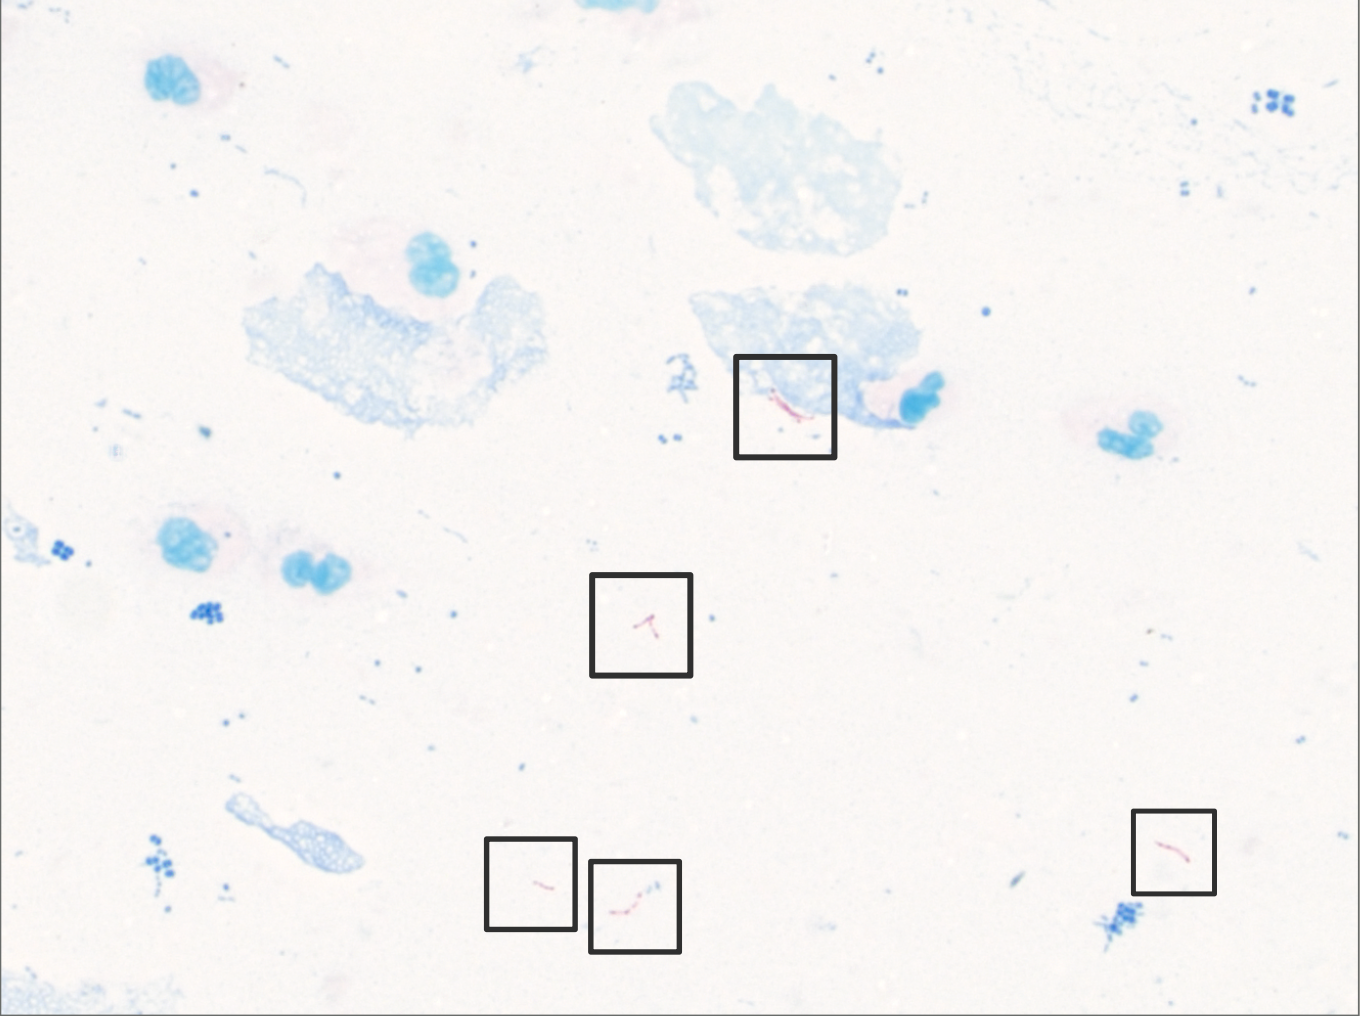
\includegraphics[width=0.9\columnwidth]{images/ODS3-Cropping.png}}
        \caption{Example of ($224 \times 224$) px croppings from ODS3, used for training the model.}\label{fig:example_cropping}
    \end{center}
    \vskip -0.2in
\end{figure}




% --- Background / Related Work ---
\section{Related Work}
% Describes what other researchers in the same area have done, and how they perhaps could be improved.

A description of similar work in the area of using machine learning models for Tuberculosis Bacilli detection
on Ziehl-Neelsen sputum smears:

\textbf{Automatic bright-field smear microscopy for diagnosis of pulmonary Tuberculosis:}
The authors of this paper also used a CNN to detect Tuberculosis\cite{Serrao2024}. They evaluated multiple architectures and even used
an encoder-decoder architecture as opposed to a generic CNN architecture, finding it to have better results.

While the authors of this paper had good success in training their model, I believe that my proposed methods are improvements
in that their crop size was much larger than mine at $(400 \times 400)$ rather than $(224 \times 224)$. A crop size of $(400 \times 400)$
not only requires a larger model to process and therefore greater computing power, but also has a greater potential of using extraneous domain
specific artifacts in its reasoning.

Further, the authors of this paper only used one dataset for their input images, choosing to strengthen their model through augmentation, while I plan to use multiple distinct
datasets in addition to augmenting my training images.


\textbf{Pulmonary Tuberculosis Diagnosis Using an Intelligent Microscopy Scanner and Image Recognition Model for Improved Acid-Fast Bacilli Detection in Smears:}
The authors of this paper were the ones who constructed the dataset the Wellgen Medical Subset was based off of\cite{chen2024pulmonary}. This study
constructed a CNN model using 100,000 sputum slides. Due to the large amount of input images, their model was able to perform
very well. However, due to it being trained on macroscopic images, rather than smaller crops like my model was, it is potentially possible that
their method generalizes worse than mine because as there is a greater chance that it uses domain specific features in its decision process, so
it might struggle when ran in foreign lab environments. Further, a CNN model trained to handle $(2448 \times 2048)$ input images would likely be
very large and computationally expensive to run, and therefore not useful in underfunded laboratories.

My method can potentially be an improvement on their method because, rather than use the entire slide as input, I extract crops which 
are easier for the CNN model to pull general and meaningful features out of and make inferences on. In addition, my model is likely much smaller
and easier to run than theirs, requires less training data to get adequate results,
and has a lesser the chance that foreign objects and image features are used in its decisions.

% https://data.mendeley.com/datasets/yhybmfrmgs/1

% https://pmc.ncbi.nlm.nih.gov/articles/PMC11356913/#_ad93_


\textbf{Automated Mycobacterium Tuberculosis Detection in Multivariant Digitized Ziehl-Neelsen Staining Using Faster R-CNN Method:}
This paper outlines training a Faster R-CNN model on the TBDB\cite{TBDB} dataset. Their methods retained the $(612 \times 480)$
image size for training their R-CNN and in addition augmented saturation, color, brightness, stretched the images, and added blur. 

There are definitely merits to the augmentations done by this team, however I believe that my model is an improvement over their methods
because my crop size is smaller, meaning my model is able to pick up on features of the small Tuberculosis Bacilli quicker than theirs, while
requiring less computational cost to run. Further, I use more diverse datasets, meaning my model is likely more robust to variations 
in lab equipment and practices and would therefore perform better in the real world.


% https://onlinelibrary.wiley.com/doi/10.1155/ijbi/6692222

% Limited in size??

% Talk about limited dataset sizes when training their models.

% --- Methodology ---
\section{Methodology}
% Describes what is the approach taken in this paper.

The main approach I used to train the CNN is to crop the dataset images from their starting resolution to a resolution
of $(224 \times 224)$ pixels around labeled Tuberculosis Bacilli. I then tested my trained model on a dataset of slides without
labels for the locations of the Tuberculosis Bacilli and made use of a custom crop viewer constructed to get an understanding of the
real world performance of my model.

I generated the $(224 \times 224)$ crops from the  training datasets using the following methods:

\textbf{ODS3 dataset:}
The Original Dataset 3(ODS3)\cite{Costa2025} is a dataset which was compiled using 3,280 extended depth focus bitmap images along with comma separated value (CSV)
files labeling the location of Tuberculosis Bacilli present on the image. The CSV uses ``b'' or ``bc'' to label bacillus
or bacillus cluster in the related bitmap image, along with coordinates for where they can be found on the image.

I cropped the bitmap format images from the ODS3 into $(224 \times 224)$ pixel crops surrounding the labeled bacillus. 
This allowed the CNN model a closer resolution to better capture the specific features of the Tuberculosis bacteria. 
Creating these crops from the labeled Tuberculosis Bacilli resulted in 10,897 images containing Tuberculosis Bacilli, labeled positive. 
I then compiled a similar number of $(224 \times 224)$ image crops without bacillus by cropping images from slides without corresponding annotation files,
these crops were labeled negative. I took 4 crops per image this way which resulted in 9,726 negative crops, roughly equal to the number of positive crops.


\textbf{TBDB dataset:}
The Tuberculosis Database (TBDB)\cite{TBDB} contains 600 $(612 \times 480)$ resolution images of Tuberculosis sputum smears along with
XML files containing bounding boxes detailing the location of the Tuberculosis Bacilli and debris on the image. 

To make this data
compatible with my model architecture, I cropped out $(224 \times 224)$ segments from these images where there was a Tuberculosis
Bacillus labeled as present. This resulted in 1,482 positive image crops. In addition, to generate negative class images which can help to train
my model against false positives, I made crops around the annotation locations which were labeled as debris and labeled the 1,585 resulting crops negative.

As the crops generated from this dataset are slightly larger than the ones generated from the ODS3 dataset, it is useful
in training the model to detect Tuberculosis Bacilli of more varying sizes.


\textbf{Testing via Wellgen Medical Subset:}
The Wellgen Medical subset\cite{lin2024tbdata} is a 1000 image subset of a large dataset of Ziehl-Neelsen sputum smear slides divided into 
$(2448 \times 2048)$ regions, released by Wellgen Medical. 

The slides in this dataset are labeled positive and negative, but none of the positive slides have bounds around the locations of the
Bacilli. As a result, I cannot use this dataset to train the CNN model. However, I found this dataset useful in getting an idea of how well my
model generalizes to data it hasn't been trained on.


\begin{figure}[ht]
    \vskip 0.2in
    \begin{center}
        \centerline{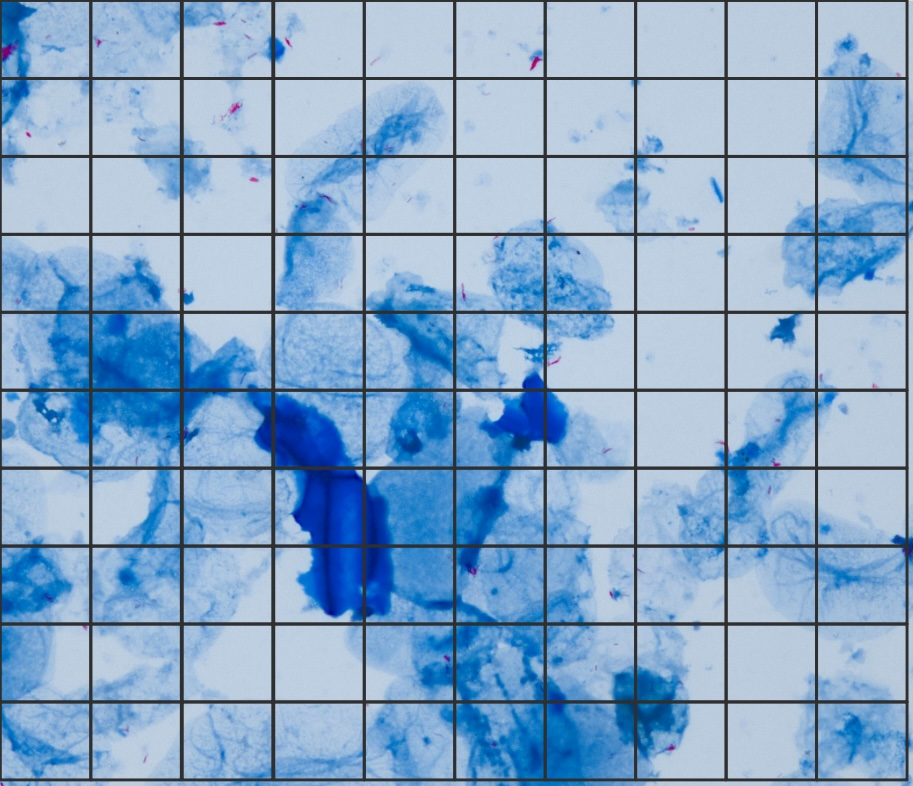
\includegraphics[width=0.9\columnwidth]{images/Wellgen_Medical_Crops.jpg}}
        \caption{Example of the 90 testing ($224 \times 224$) px croppings taken from a positive slide with no location labels.}\label{fig:wellgen_cropping}
    \end{center}
    \vskip -0.2in
\end{figure}


Specifically, to test models using the images in this dataset I separate the $(2448 \times 2048)$ images into 90 $(224 \times 224)$ crops (See Figure 2). 
I then have the model being tested predict the probability that Tuberculosis Bacilli are present in each of the crops and
if the probability is greater than a threshold of 0.5 I count the crop as being positive for Tuberculosis. I then sum up all of the positive
crops for a slide and if more than half of the crops are counted positive I label the slide as positive. I run this for all 100 of the positive slides
in the dataset and a subset of 100 of the 1000 negative slides in the dataset.

% I calculate two values using this dataset, the percentage of slides marked as positive/negative and the total number of positive/negative slides.
I've found the expected values for a well performing model differ based on whether the slide is positive or negative. A well performing model will
 be able to classify most or all 9000 of the crops from the negative slides as negative, however a well performing model should not classify all 9000
of the positive crops as positive. This is because on the positively labeled slides, only about 5--20\% of the cropped fields actually appear to 
contain Tuberculosis. Therefore the percentage of positively labeled slides will be fairly low and the total number of positively predicted crops should 
be around 1000--2000 crops.


While this testing methodology is not perfect, it does give fairly good insight into how well the model is able to sort the croppings by their likelihood,
which is the ultimate goal of this project.

% further evidenced by the use of a dataset (Wellgen Medical) which appears to contain images with a wider variety of staining intensity and
% visual artifacts. 


% pipeline: transform images into $224 \times 224$ crops. run model on each of the crops. count total number
% of positive classifications, multiply assurances to get average assurance for image.
% sum together all trials for all slides. divide by number of slides? achieved an accuracy metric which should
% be similar to percentage of positive vs negative?? 

\textbf{Crop Likelihood Viewer:}
To allow for manual validation of the model's performance a tool was constructed to visually sort a sputum slide by the likelihood of the 
presence of Tuberculosis Bacilli. This tool displays the various cropped view fields, sorted from most likely to contain TB to the least
likely, as well as the total numbers and percentages of the positively and negatively predicted crops from the slide (See figure 3).

\begin{figure}[ht]
    \vskip 0.2in
    \begin{center}
        \centerline{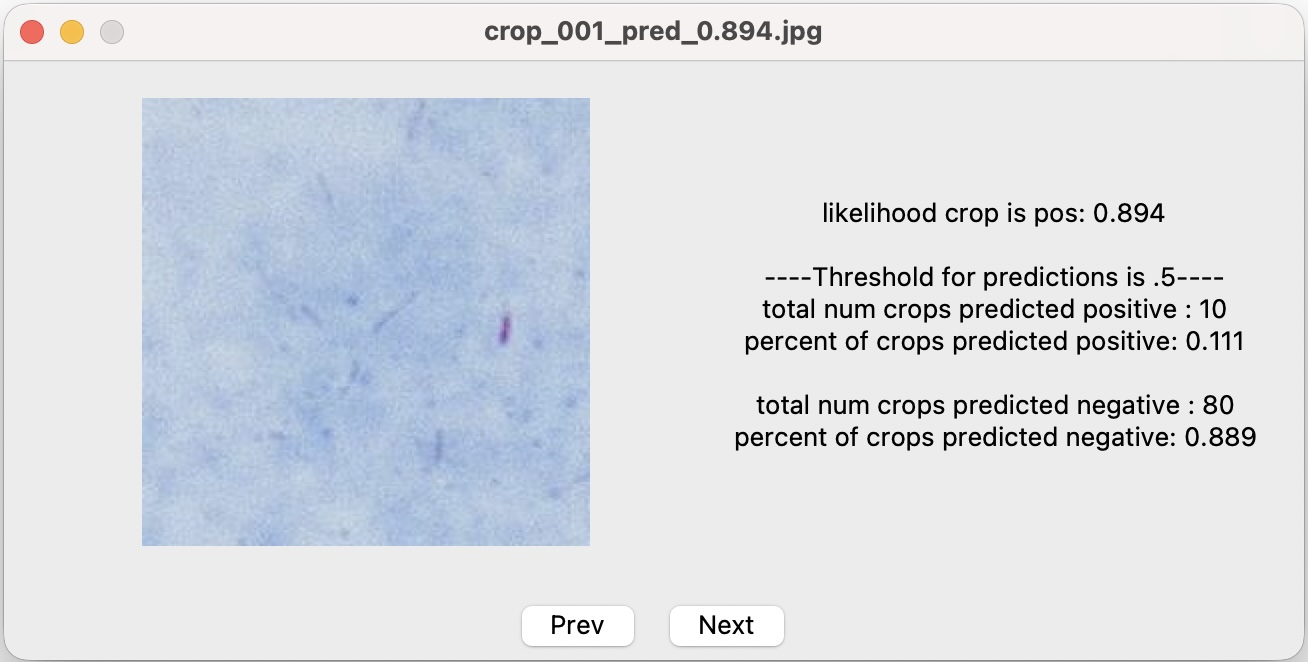
\includegraphics[width=0.9\columnwidth]{images/Sample-Tool.jpg}}
        \caption{TB likelihood imaging tool.}\label{fig:sample_tool}
    \end{center}
    \vskip -0.2in
\end{figure}


% --- Experiments ---
\section{Experiments}
% Describes the experiments performed, including details on the data used.
% model architecture—pooling layers, dense layers, convolutional layers

% ????	Convolutional filters, hidden layers, activation functions for each node ?????

I used the Keras implementation as a baseline for my CNN, with a $(224 \times 224 \times 3$ channel) input schema, Binary Cross Entropy Loss,
the Adam optimizer, the ReLU activation function for the convolutional layers, a sigmoid activation for the output layer, and a learning rate of 1e-4.

Further, the input images were split into a validation set and a training set via a 20/80 split respectively 
and normalized by dividing their pixel values by 255.

\textbf{Training with only ODS3:}
I began my experiments working with my cropped modification of the ODS3 dataset to find a viable model architecture. I chose to being
working with only ODS3 because it was the larger of the two training sets I had and it 
contains slides with less visual artifacts and staining distortion. I wanted to get my model
working on a baseline input set, before I would look into attempting to improve generalization performance.


In my investigation, I found that the model appeared to overfit this dataset very early on in the training process.
I attempted to combat this by selecting a simplistic architecture with a low number of filters and few convolutional layers,
but then found that said architecture appeared to not be complex enough to converge well.

Ultimately, the best architecture I found for this dataset was 5 convolutional layers, interspersed with (2,2) max pool layers, starting
from in the pattern of (64, 64, 128, 128, 256) convolutional filters.

This architecture achieved a validation accuracy of 0.9092 and a validation loss of 0.2901. By these results, the model can be said
to be a fairly good classifier for the data, but it still needed to be tested with other datasets and on my testing set.


\textbf{Augmenting with TBDB and constructing a Wellgen generalizable model:}
Once I included the TBDB data into my training and evaluation, I found that my model began to struggle to accurately classify with
low loss. This is likely due to the fact that the TBDB images were at a higher resolution, so my $(224 \times 224)$ crops caused the
Tuberculosis Bacilli to appear enlarged compared to the ODS3 images.

While this increased the training difficulty, I believe it is necessary to train on both of these sets as I am hoping to 
produce a generalizable model which can be used in many different lab environments where imaging setups might have different 
microscope magnification. 

Further, the images in the Wellgen Medical subset, my testing set, are also captured from a third different
lab environments, requiring even more generalization power from the model.
To attempt to further increase my model's generalization I added an augmentation layer that runs every epoch and augments
the training images, but not the testing images.

In this augmentation layer I added random flips and random rotations, zooms, brightness, and contrast operations with a factor of 0.4.
These augmentations greatly decreased the likelihood my model overfit its training data,
but also made training more difficult and added greater computationally complexity.

Finally, I added batch normalization between my convolutional layers and my activation layers to further reduce the complexity
of my weights. I also added dropout layers after the first and second max pooling layers with factors of 0.2 and 0.1 respectively
and another final dropout layer with a factor of 0.5 after my global max pooling layer and before my final output activation. These
dropout layers further reduced overfitting and the likelihood of having few convolutional filters capable of detecting important features.


With this setup I found the most performant model to be 5 convolutional layers, each with $(3 \times 3)$ kernels and increasing
filter amounts of $(32, 32, 64, 64, 128)$ and respective max pooling layers of size ($2 \times 2$) after the first three convolutional layers 
which gradually decrease model complexity, but still allow for downstream feature extraction (See Figure 4).

\begin{figure}[ht]
    \vskip 0.2in
    \begin{center}
        \centerline{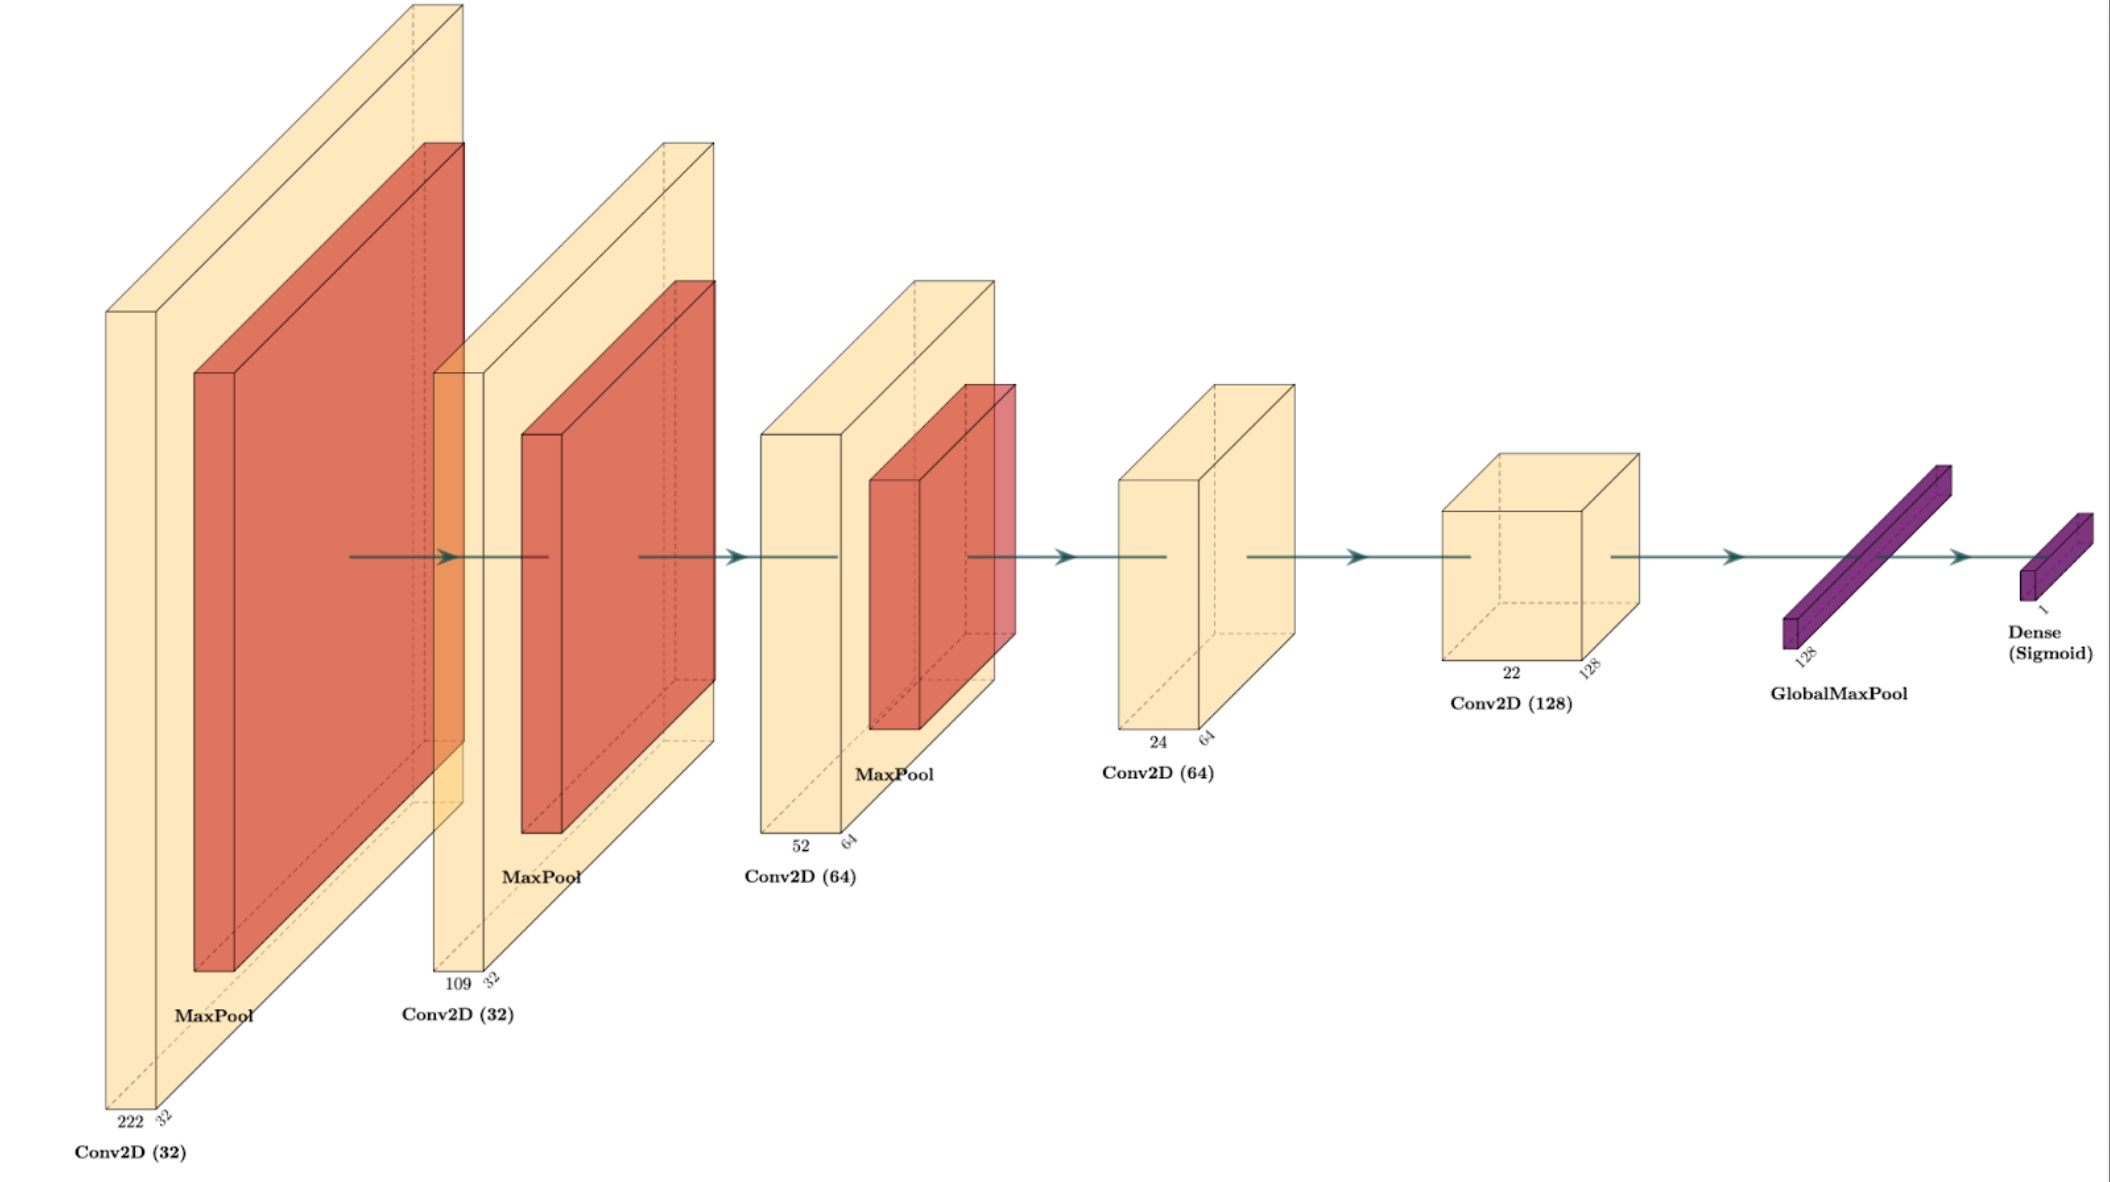
\includegraphics[width=0.9\columnwidth]{images/Model_Architecture.jpg}}
        \caption{Final constructed model architecture.}\label{fig:wellgen_cropping}
    \end{center}
    \vskip -0.2in
\end{figure}


% \begin{center}
% 
\includegraphics[scale=.25]{SimpleTrainingSetup.png}
% \end{center}

% \textbf{Identifying Number of Epochs:}
% First, I wanted to select an appropriate number of epochs to prevent overtraining and limit
% the amount of time spent training a model.

% Training the CNN for 100 epochs resulted in the following graph:

% \begin{center}
% 
\includegraphics[scale=.25]{SimpleTraining100Epochs.png}
% \end{center}

% Based on the divergence of the training accuracy versus the validation accuracy it appears that 20
% epochs is sufficient to to achieve the best training results while minimizing the time spent overfitting.
 

% 
\includegraphics[scale=.4]{20EpochsView.png}

% \textbf{Drafting CNN Architecture to Minimize Loss:}
% Using my initial CNN configuration I achieved a validation accuracy of 0.8264 and a validation loss of 0.4319.


% While the accuracy is fairly high, a loss of 0.4319 shows that the model is uncertain about the validity of its predictions.

% I increased the number of filters for the first convolutional layer to 64, this would hopefully
% allow me to capture the shape of the small Bacilli more accurately from the beginning
% I also lowered the kernel size from (3,3) to (1,1) to try and understand how the size of the kernel affects detection. 

% 
\includegraphics[scale=.4]{FirstExperimentalModification.png}
% 
\includegraphics[scale=.4]{FirstExperimentResult.png}

% This experiment resulted in a validation accuracy of 0.8992 and validation loss of 0.2958. Simply from the change in architecture, both validation 
% accuracy and loss have greatly improved. 

% To further increase accuracy and decrease loss I tried the model with 128 filters on the first 
% convolutional layer. This change resulted in a validation accuracy of 0.8938 and a validation loss of 0.3129.



% 
\includegraphics[scale=.4]{Experiment2_128FeatureStarting.png}
% 
\includegraphics[scale=.4]{128FilterStart.png}


% Because of the significant increase in training time and slight decrease in accuracy, I then decided to evaluate 
% starting with less features in the first few layers and attempt to increase features as I downsample. 


% Shifting to a model which gradually applies more and more filters as it slowly downsizes:
% \begin{center}
% 
\includegraphics[scale=.25]{FirstGradualTrainingModel.png}
% \end{center}

% 
\includegraphics[scale=.4]{FirstGradualTrainingModelGraph.png}


% This architecture resulted in a validation accuracy of 0.8606 and a validation loss of 0.3823, which are both a downgrade 
% from the previous method.

% These results led me to believe that my model was not complex enough and therefore could not capture an adequate hypothesis which would
% allow it to fit the data well. Because of this I decided to start at 64 filters rather than 32 and added another convolutional layer and max pooling
% layer both with 256 filters.

% \begin{center}
% 
\includegraphics[scale=.3]{32Start256End.png}
% \end{center}

% 
\includegraphics[scale=.4]{32Start256EndGraph.png}

% This combination resulted in a validation accuracy of 0.9092 and a validation loss of 0.2901 which is the best accuracy and
% smallest loss I have gotten yet while still having a reasonable training time.

\textbf{Experimental Results:}
The increased model size and variability caused the convergence time to greatly increase, but the model also gained a much greater
ability to generalize.

Training based on the architecture described above took about 12 hours of training time and 100 epochs to effectively converge. The augmentation layer applied
to the training set caused deviations to appear in the observed loss, but overall the results are conducive to an effective
convergence. 

The minimum validation loss observed was 0.2097. This validation loss is low enough that it shows the model generalizes fairly well to unseen
data, but there is certainly room for future improvement.  


\begin{figure}[ht]
    \vskip 0.2in
    \begin{center}
        \centerline{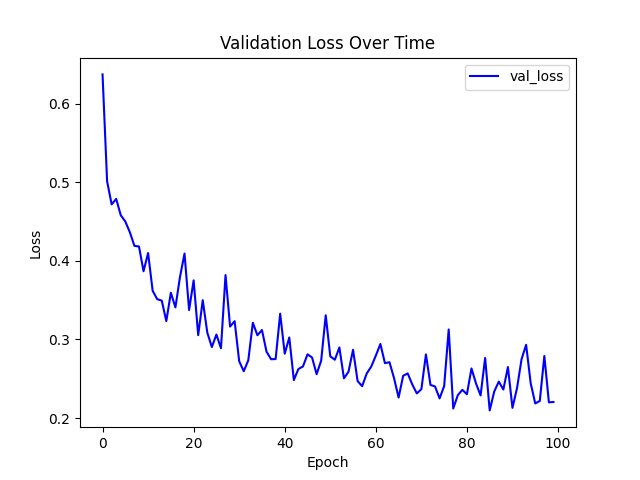
\includegraphics[width=0.9\columnwidth]{images/final_loss.png}}
        \caption{Graph of the validation loss from the 100 epoch run.}\label{fig:final_loss}
    \end{center}
    \vskip -0.2in
\end{figure}

After 100 epochs, the training successfully achieved a 0.9198 validation accuracy. This accuracy score is quite high and 
is indicative that not only can the model be applied to unseen data, it can be used to accurately classify unseen data as well. 

Similarly to the effect seen in the loss, the dropout layers caused spikes in the validation accuracy compared to the training accuracy.
However, the spikes in the validation accuracy have a consistent deviation and still show gradual a gradual increase over time
as training continued (See Figure 6). 

\begin{figure}[ht]
    \vskip 0.2in
    \begin{center}
        \centerline{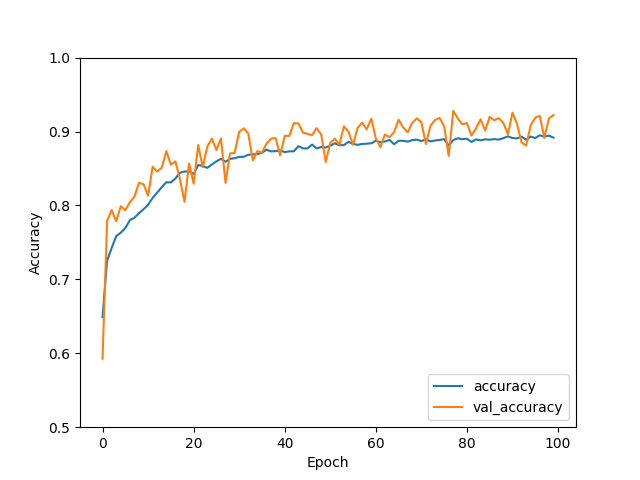
\includegraphics[width=0.9\columnwidth]{images/final_accuracy.png}}
        \caption{Graph of the training and validation accuracy from the 100 epoch run.}\label{fig:final_loss}
    \end{center}
    \vskip -0.2in
\end{figure}


Finally, training for 100 epochs showed approximate convergence in the classifications of the crops from the positive and negative
slides of the aforementioned Wellgen Medical subset used for testing. 

As previously mentioned, the model was tested by taking 90 crops from both
100 positive slides and 100 negative slides for 9000 crops total for each class. Crops with an output likelihood of over a 0.5 probability threshold were counted as positive, 
while the ones under the 0.5 threshold were counted as negative.

The results from the classifications show the model was able to perform quite well in the classification task at later epochs. 
Because there are no tuberculosis found on negative slides it is expected a well performing model will classify around 9000 of the negative crops
as negative. This was seen in the model's performance at later epochs. At the epoch with the best reported validation loss, the number of negative crops
was 8836, this is very close to the target of 9000, thus providing evidence that the model is able to classify slides not containing TB quite well.

Accuracy interpretation is more complicated when it comes to the positive class. The positive slides tested tend to range from having about
5--20\% of their croppings containing Tuberculosis Bacilli. Because of this, a well performing model should report somewhere between $1000-2000$
slide crops as positive from the 9000 tested positive slides, and report the rest as negative. At the epoch with the best reported validation loss, the number of positive
crops detected was 1134. This number of positive crops is within the expected range, thus providing further evidence for the model generalizing well (See Figure 7).


\begin{figure}[ht]
    \vskip 0.2in
    \begin{center}
        \centerline{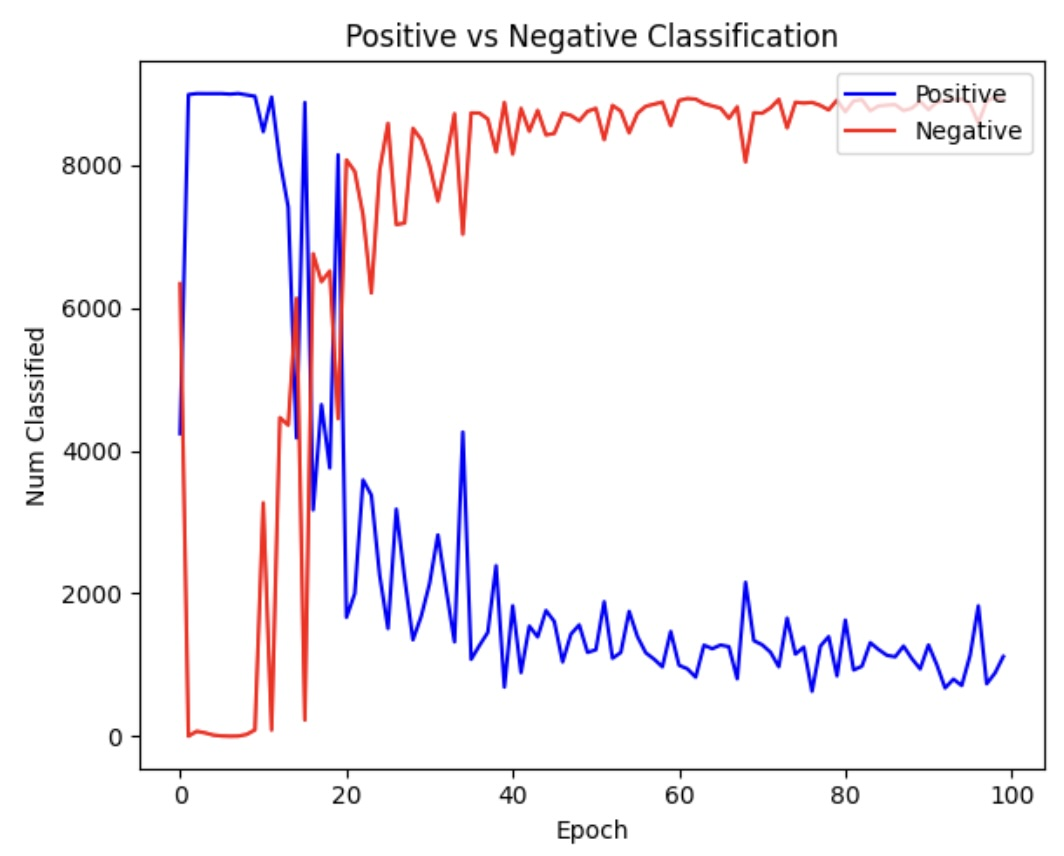
\includegraphics[width=0.9\columnwidth]{images/positive-negative-classification.jpg}}
        \caption{The number of positive and negative classifications over the 100 epoch run.}\label{fig:final_classifications}
    \end{center}
    \vskip -0.2in
\end{figure}





% Best Results:

% testing sub croppings of slides labeled positive:
% total amount of crops predicted positive: 1134
% percent slides predicted positive: 0.07
% testing 9000 negative slide crops


% testing sub croppings of slides labeled negative:
% total number of crops predicted negative: 
% percent of slides predicted negative: 1.00


% While it is acceptable to use the validation set to search for an appropriate group of hypothesis classes, which in this
% case it would be the structure of the network, it is not adequate to use the validation set to estimate the model's overall 
% performance.

% To approximate the classification power of the model I will be using the previously described test set of Ziehl-Neelsen slides which contains
% images that none of the models were trained on. The accuracy threshold I will be using to evaluate my probabilities is 0.80

% With my latest model I achieved a positive prediction rate of 0.53 and a false-positive prediction rate of 0.45.

% These numbers show that the model is doing a very poor job at correctly detect Tuberculosis bacterium and major improvements still need
% to be made before the model is viable.

% The high testing accuracy and low real-world accuracy of my model lead me to believe that my data was overfitting. So, because simpler models 
% are less prone to overfitting I reduced the amount of filters present in my model.
% However, at the same time I increased the number of layers believing that with the additions of more layers my model will still able to 
% fit the data well.

% This following architecture achieved a positive prediction rate of 0.93 and a false-positive prediction rate of 0.44:

% \begin{center}
% 
\includegraphics[scale=.25]{SimplifiedLessWeightsMoreLayers.png}
% \end{center}

% The results are beginning to look favorable, to push my model even further I decided to increase the number of negative examples in my modified ODS3 training set
% so it was closer to the number of positive values. 

% This modification to my training set resulted in a positive prediction rate of 0.98 and a false-positive prediction rate of 0.68. This large bias to the positive 
% led me to simplify my model even more, resulting in the following configuration:
% \begin{center}
% 
\includegraphics[scale=.25]{EvenSimplerModel.png}
% \end{center}

% This configuration resulted in a positive prediction rate of 0.89 and a false-positive prediction rate of 0.41, much more distributed from each other,
% but still showing that the model is having a hard time accurately detecting negative classes. 

% To further improve my model I will randomize my crops every 5 epochs, this will prevent overfitting based on location and will help the model learn
% features like the shape of the Bacilli and size. 




% Also, I will augment the dataset with the TBDB dataset to help the model learn variations in size
% of the bacteria, as the Bacilli in the TBDB appear slightly larger than they do in the ODS3 dataset.

% Finally, I will add images with varying saturation, color, brightness, stretched the images, blur similar to the process that
% Trilaksana et al. underwent with their model to further improve my model's generalization power.





% --- Discussion / Analysis ---
\section{Discussion and Feature Analysis}
% Examines the results of the experiments and draws some conclusions about their significance.
\textbf{Discussion:}
Detecting Tuberculosis via Ziehl-Neelsen microscopy is currently the cheapest and most accessible Tuberculosis 
diagnostic technique but is also very time-consuming and prone to false negatives. Because
of this, a tool that can accurately flag areas with high potential for Tuberculosis presence and can then present them 
to be reviewed by a trained technician is highly useful.

 Such a tool could be operated relatively inexpensively but greatly increase the rate of
Tuberculosis detection and the speed of a diagnosis, cutting down the time technicians spend searching for bacterial presence on a slide. 
Not only would such a tool help a technician achieve better diagnostic results, speeding up the diagnostic time
also means potentially freeing up time for other patients' sputum slides to be analyzed, increasing the overall rate of patient diagnostics.


% \textbf{Analysis:}



\textbf{Feature Analysis:}
The model appears to use features such as color, shape, and depth in its analysis. In images derived from the various convolutional layers it
appears the filters are able to extract the three dimensionality of the bacilli in relation to the two dimensional slide they appear on (See Figure 8). 

Further,
I have noticed that the model performs better when there is a darker pink stain on the bacilli as opposed to bacilli stained with a less intense pink,
leading me to believe that color is an important feature in detection as well. 

Finally, it appears the shape of the bacilli is useful as the model is able to distinguish 
stained debris from actual bacilli with fairly good accuracy.



\begin{figure}[ht]
    \vskip 0.2in
    \begin{center}
        \centerline{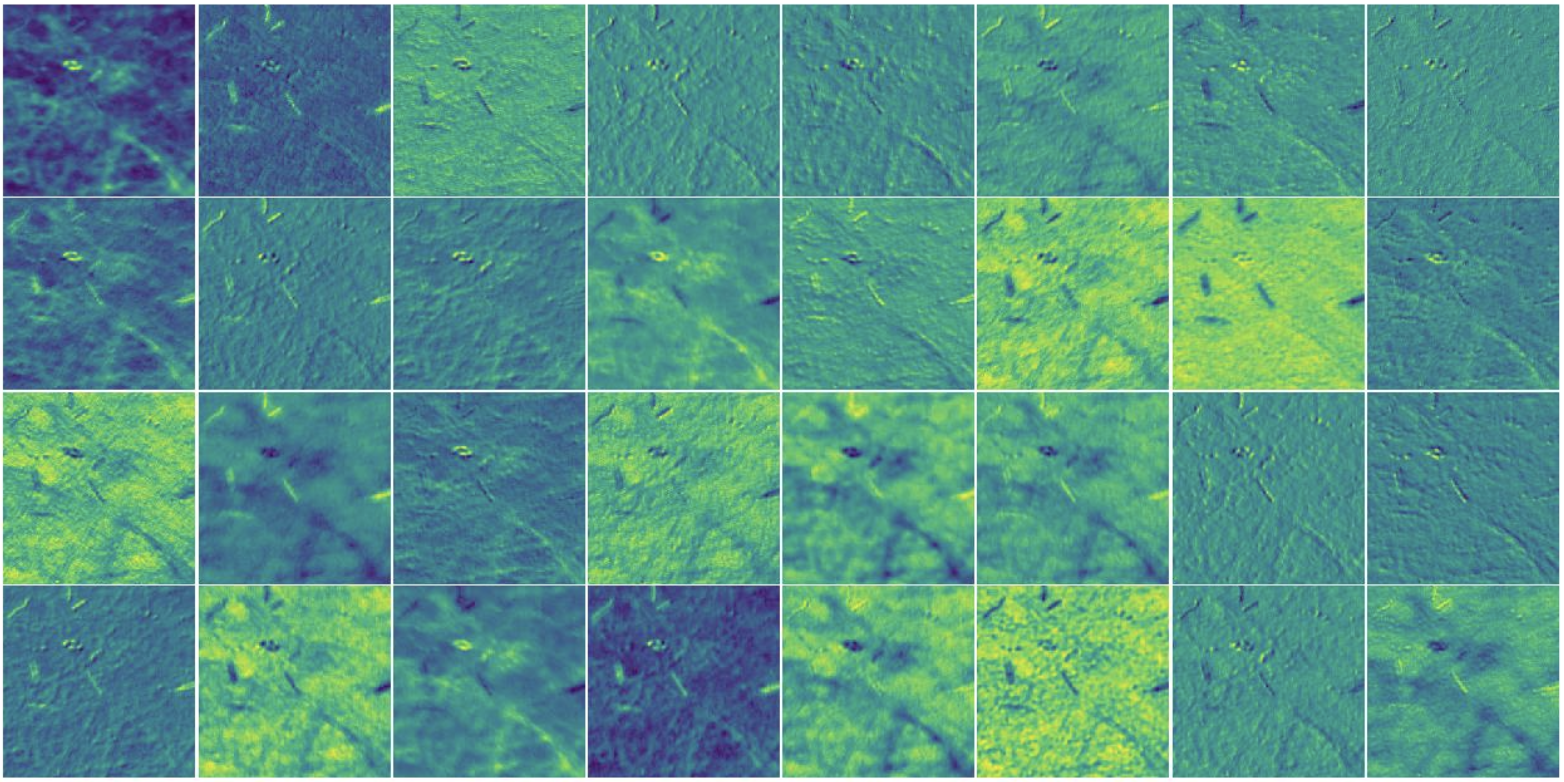
\includegraphics[width=\columnwidth]{images/Conv-Filter-Image.jpg}}
        \caption{Visualization of the filters from the first convolutional layers, 
        input image crop was predicted positive with a likelihood of 0.985.}\label{fig:conv-filter-visualization}
    \end{center}
    \vskip -0.2in
\end{figure}


% --- Conclusion ---
\section{Conclusion}
% Summarizes the paper.

The problem of detecting Tuberculosis is difficult because the places where it is most prevalent also lack adequate healthcare funding to do something about it.
The most accessible diagnostic tool in the poorer regions where Tuberculosis is highly infectious is Ziehl-Neelsen stained slide microscopy. Microscopy is 
cheap and therefore accessible, but requires trained technicians to spend hours looking through microscope lenses to diagnose a single patient. 

The classification system proposed in this article would be able to greatly speed up the rate at which a technician is able to classify Tuberculosis Bacilli by presenting areas of a
viewfield to the technician where there is the greatest likelihood of Tuberculosis being present.

% \section{Future Work}

% --- Bibliography ---
% \section{Bibliography}
% Gives properly formatted references to other scholarly work that
% this work is built on. Note that the references should be scholarly, which means things 
% like refereed conference and journal articles. Importantly, that rules out things like 
% most websites, basic textbooks, and press articles.

\bibliography{../references/references} % This looks for a file named references.bib
\bibliographystyle{../style/icml2025}


\end{document}